\section{Method}
       To assess how task homogeneity and interdependence affect human experience with collaborating with a robot, we simulated a manufacturing workcell using a robotic arm and an experiment task inspired by real-world manufacturing operations.  We asked participants to perform multiple rounds of the manufacturing task, and measured their perceptions of the robot as well as the collaboration.
\subsection{Study Design}
       The study followed  a $2\times2$ between-participants design involving two factors-task homogeneity and task interdependence, resulting in four unique experimental conditions: (1) non-homogeneous, non-interdependent; (2) non-homogeneous, interdependent; 3) homogenous, non-interdependent and 4) homogeneous, interdependent. The conditions are described in greater detail in the following paragraphs.

\subsection{Experiment Setup, Materials, and Tasks}
\subsubsection{Collaborative Robot Platform}
       To create a simulated hybrid, human-robot workcell, we utilized a Kinova Mico robotic arm-a lightweight underactuated multipurpose robotic arm (shown in Figure 1). The arm has six degrees of freedom with unlimited rotation on each axis and a gripper with two fingers that can be used to grasp, manipulate, transport, and release objects. We programmed the robot to perform a manufacturing task using the Robot Operating System (ROS) application programming interface (API). The robot's actions and behaviors in each experimental condition were pre-programmed, and the robot followed a specific schedule for that condition.
\subsubsection{Workspace Setup}
        We simulated a single-station hybrid manufacturing workcell in our laboratory (also shown in Figure 1). The robotic arm was installed on the workbench at a distance that allowed it to share a task with its human collaborator while minimizing any potential safety risks to the participant. The robot and human workers were each given an inventory shelf that contained parts that were required for the manufacturing tasks described below. The robotic arm could re-stock its shelf or take parts from it. The human will take parts from his shelf. The  conveyor belt where the workers would place assembled materials to be delivered to the next hypothetical station was simulated using tapes placed on the workbench. Empty boxes required for the task were stacked on a pallet next to the workbench.
\subsubsection{Task}
       To achieve a realistic simulation of a manufacturing workcell in our laboratory, we developed a manufacturing task that subsequently integrated two real-world manual manufacturing operations: kitting and stocking. Kitting is a process in which several loose parts are placed in a box or container. In a complex workcell, the kit may be used to assemble parts in the next station or workcell  or may be assembled into a final product that will be shipped to the customer.  Stocking is a process by which parts or completed products are stocked, piled up, or put on a shelf for future use. For example, parts may be stocked on a shelf, and a different  worker may pick them up to assemble a product or to produce a kit. Final products may also be stocked prior to be shipment to customers. Both operations were selected and integrated into a task that could be performed individually by a human or a robot worker or collaboratively by a human-robot team.\\
       In the task, the robotic arm and/or the human worker assembled small toy lanterns shown in Figure 1. Each lantern was composed of a body, base, battery cap, light cover, and one screw. This product offered an appropriate level of complexity for individual and collaborative assembly and involved parts that can be manipulated by both human and robot given the state-of-the-art technology.  The “kit” included four lanterns placed in a cardboard box and securely fitted into an insert.
\subsection{Experimental Conditions}
      We manipulated  the manufacturing task described above to create the following four conditions that involved different levels of task interdependence and homogeneity for a human-robot team:
\subsubsection{Non-homogeneous, non-interdependent} In this condition, the robot and the participant worked on different tasks that did not depend on each other.  Specifically, the robot performed stocking while the participant performed kitting, resulting in non-homogeneous tasks, and the robot stocked parts on the shelf that were not relevant to the kit that the participant was producing, resulting in non-interdependent tasks. In the task, the participant picked up a box, then picked up the body, base, and battery cap from the shelf, and put these parts in the box. The task required the participant to place the screw and light cover in a small plastic bag and to put the bag in the box. The box was then placed on the conveyor belt.
\subsubsection{Non-homogeneous, interdependent} In this condition, the robot and the participant similarly worked on different tasks, stocking and kitting, resulting in  a non-homogeneous task allocation. However, their tasks were dependent such that the parts that the robot stocked would be used by the participant for producing the kit. Specifically, the robot took the lantern body from its own shelf and stocked it on the desk for the participant to retrieve. This process is similar to Condition 1 except that the participant manipulated the body from the pile that robot had stocked.
\begin{figure}
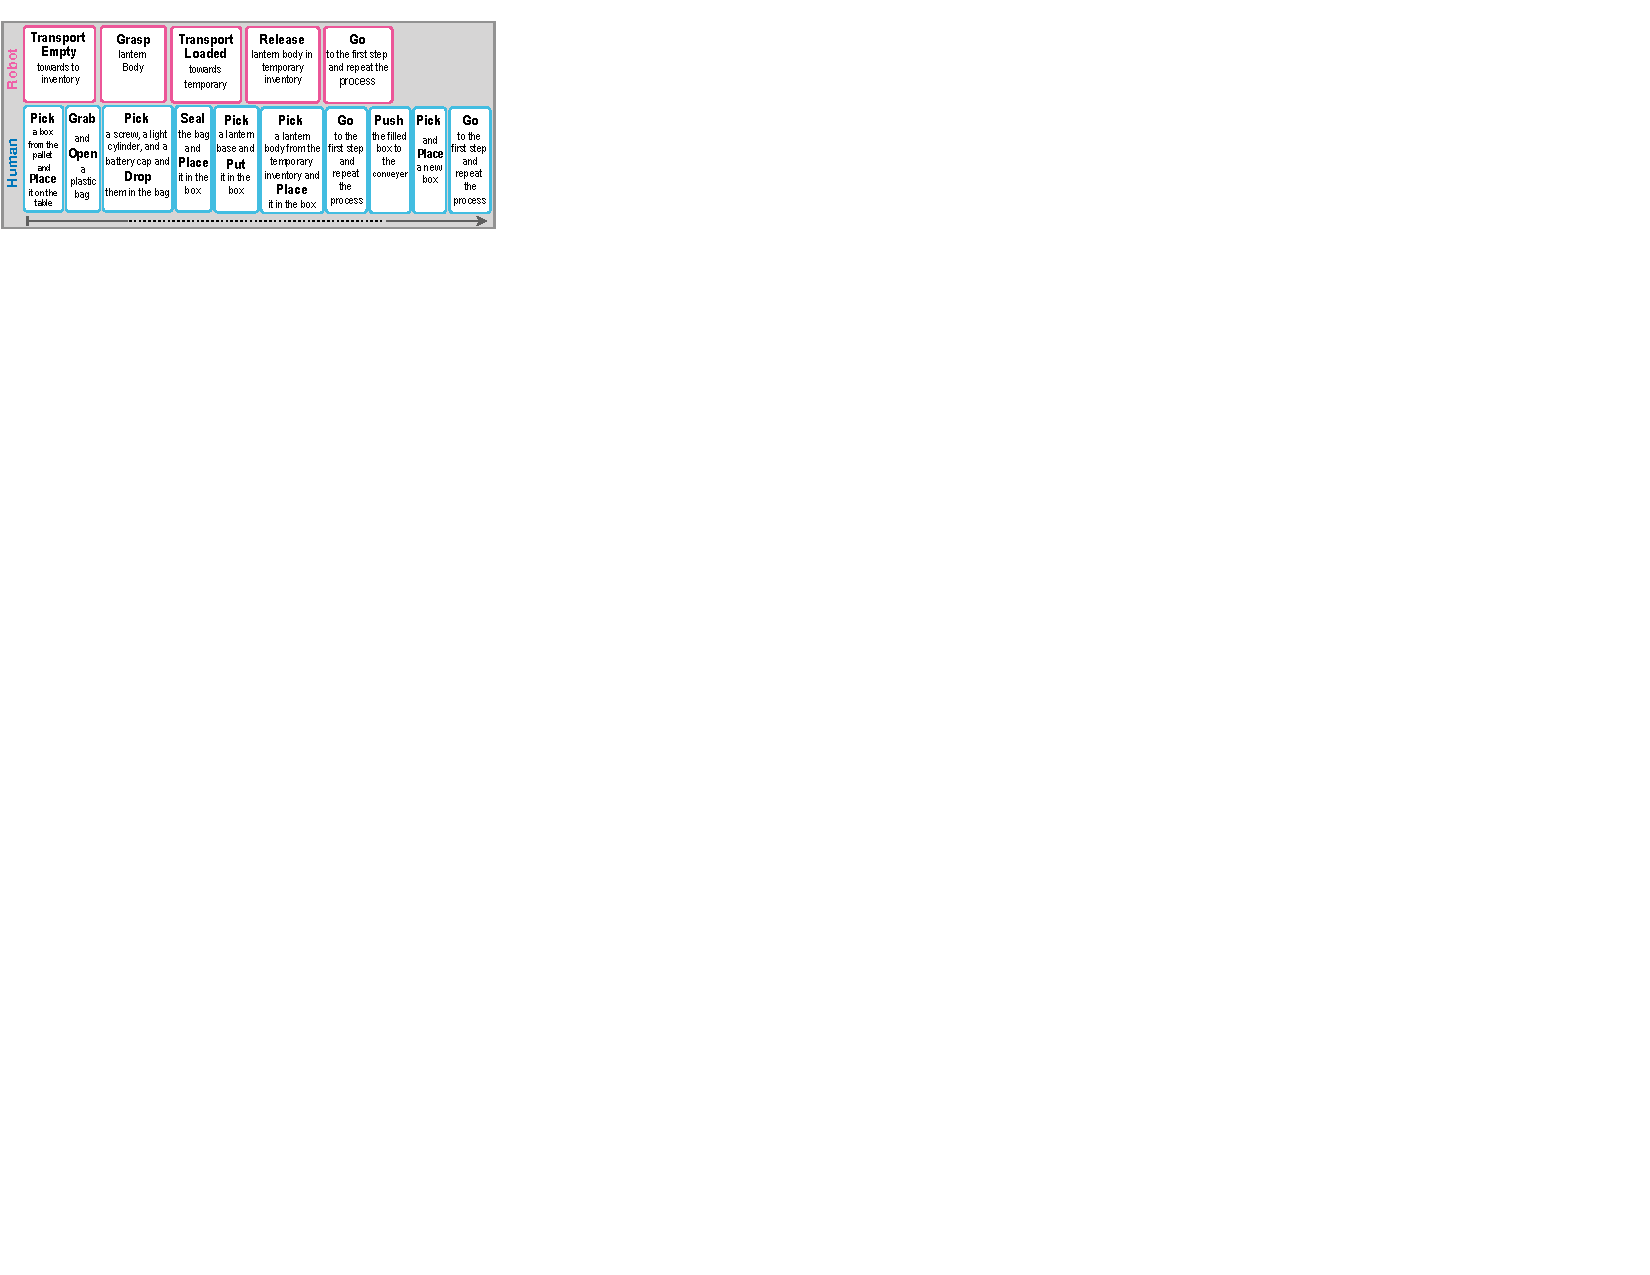
\includegraphics{condition2}
\caption{A sample black and white graphic
that needs to span two columns of text.}
\end{figure}
\subsubsection{Homogeneous, non-interdependent} In this condition, both the robot and the participant performed kitting, resulting in homogeneous tasks for the two workers, in a non-interdependent fashion. Specifically, the robot produced a complete kit by itself, and the participant produced a complete kit by himself or herself. They both placed the boxes on the conveyor once kitting was complete.
\subsubsection{Homogeneous, interdependent} In this condition, both the participant and the robot performed kitting in a homogeneous task setup. Their work depended on each other. In particular, the robot picked a body from its shelf and placed it inside the box that the participant was also filling with parts. Similar to the previous conditions, the participant picked up the remaining parts from the shelf and placed them in the box. The participant then placed the box on the conveyor belt.
\subsection{Procedure}
       After informed consent, a male experimenter led the participant to the simulated manufacturing workcell. The experimenter then showed the participant an instructional video that demonstrated a human and the robot collaboratively working according to the particular condition to which the participant was assigned in order to establish familiarity with the task. The experimenter then showed to the participant the different elements of the workcell, such as the robot, the shelves, the empty boxes, and the conveyor belt. The participant was then asked to assemble a single kit as a trial run. The experimenter then started the experiment and left the workcell. After assembling five kits, the participant was directed to a computer to complete the first questionnaire designed to measure participant demographics. After the first questionnaire,  the participant was directed back to the workcell and asked to assemble five more kits, followed by a second questionnaire that measured subjective aspects of the participant\' s experience with the robot and the task. After the questionnaire, the experimenter administered a brief semi-structured interview, debriefed the participant, and provided compensation. The experiment was video-taped for future analysis. Each participant trial took approximately 30 minutes.
\subsection{Participants}
       The study included 32 participants (16 males, 16 females) recruited from the University of Wisconsin-Madison campus. Participant ages ranged from 18 to 35 (M = 22.65, SD = 4.15).
Twenty-one participants were native English speakers. Participants were from a variety of backgrounds, including as Geography, Computer Sciences, Mathematics, and Microbiology. Participants reported low familiarity with robots and manufacturing (M = 3.06, SD = 1.66, M = 3.37, SD = 1.63, respectively, on a seven-point rating scale).
\subsection{Measures}
       In order to measure participant experience with human-robot collaboration under four conditions described above, we used a self-report questionnaire and a semi-structured interview administered after the experiment.
\subsection{User-Experience Questionnaire}
       We constructed Likert scales to measure participant experience with the robot, including perceived competence of the robot, perceived contribution of the robot, how the robot's presence affected participant work, perceived enjoyment of working with the robot, and perceived collaboration with the robot. We refer to these as competence, contribution, presence, enjoyment, and collaboration, respectively, hereafter. Items included in these measures are shown in Table 1. We also measured participants\' physical and cognitive workload using the NASA Task Load Index (TLX) \cite{hart1988development}, which has been validated to provide consistent and reliable measurement of task load across various tasks \cite{hart2006nasa}. Participant responses were measured using a seven-point rating scale for all scale items.
 
 %===============================      
\begin{table*}[]
\centering
%\caption{My caption}
%\label{my-label}
\begin{tabular}{ll}
\hline
\multicolumn{2}{|l|}{\textbf{User Experience Questionnaire}}                                                                                                                                                                                                                                                                                                                                                                                                                               \\ \hline
\multicolumn{1}{|l|}{\textbf{Competence}}      & \multicolumn{1}{l|}{\begin{tabular}[c]{@{}l@{}}1. I trusted that the robot would perform its task correctly.\\ 2. I was confident about the robot’s work.\\ 3. I thought that the robot was reliable.\\ 4. The robot knows what it is doing.\\ 5. The robot is smart.\\ 6. The robot was competent in performing the task it was assigned.\\ 7. The robot has a sophisticated program controlling its actions.\end{tabular}}              \\ \hline
\multicolumn{1}{|l|}{\textbf{Task Load Index}} & \multicolumn{1}{l|}{\begin{tabular}[c]{@{}l@{}}8. How mentally demanding was the task?\\ 9. How physically demanding was the task?\\ 10. How hurried or rushed was the pace of the task?\\ 11. How successful were you in accomplishing what you were asked to do?\\ 12. How hard did you have to work to accomplish your level of performance?\\ 13. How insecure, discouraged, irritated, stressed, and annoyed were you?\end{tabular}} \\ \hline
\multicolumn{1}{|l|}{\textbf{Presence}}        & \multicolumn{1}{l|}{\begin{tabular}[c]{@{}l@{}}14. I could easily predict the next movement of robot.\\ 15. Trying to pay attention to the robot’s movements was stressful.\\ 16. I found myself being distracted by the robot’s movements.\\ 17.The robot got in my way while I did my work.\\ 18. The robot’s presence did not affect my work at all.\end{tabular}}                                                                     \\ \hline
\multicolumn{1}{|l|}{\textbf{Contribution}}    & \multicolumn{1}{l|}{\begin{tabular}[c]{@{}l@{}}19. I found the robot to really contribute to the task.\\ 20. It would have been harder to do the task without the robot.\\ 21. Having the robot’s contribution made the task easier.\\ 22. Working with the robot made my work easier.\end{tabular}}                                                                                                                                      \\ \hline
\multicolumn{1}{|l|}{\textbf{Enjoyment}}       & \multicolumn{1}{l|}{\begin{tabular}[c]{@{}l@{}}23. I enjoyed working with the robot.\\ 24. Working with the robot made the task enjoyable.\end{tabular}}                                                                                                                                                                                                                                                                                  \\ \hline
\multicolumn{1}{|l|}{\textbf{Collaboration}}   & \multicolumn{1}{l|}{\begin{tabular}[c]{@{}l@{}}25. I would prefer to perform this task without the robot.\\ 26. I prefer working with a human in this task instead of the robot.\\ 27. I enjoyed collaborating with the robot in this task.\\ 28. The robot and I make a good team.\end{tabular}}                                                                                                                                         \\ \hline
%\multicolumn{2}{l}{Table 1: User experience questionnaire that consisted of five scales to measure participant experience with the robot: Competence, Task Load Index, Presence, Contribution, Enjoyment, and Collaboration.}                                                                                                                                                                                                                                       
\end{tabular}
\caption{User experience questionnaire that consisted of five scales to measure participant experience with the robot: Competence, Task Load Index, Presence, Contribution, Enjoyment, and Collaboration.}
\label{my-label}
\end{table*}
